\section{Schätzen \skript{127} \sachs{134}}

	\subsection{Konsistente Schätzer \skript{129} \sachs{136}}
		Ein Schätzer ist konsistent, wenn $\lim \limits_{n \rightarrow \infty}$ = E(X)
		ergibt\\
		\begin{tabular}{p{10cm}p{8cm}}
        Der Mittelwert der Stichprobe ist ein konsistenter Schätzer.
        & $\lim\limits_{n\to\infty}=\frac{X_1+\ldots+X_n}{n}=E(X)$
        \end{tabular}

        \hspace*{2.1mm}Der Schätzer $\bar{X}=\frac{X_1+\ldots +X_n}{n}$ heisst
        der Stichprobenmittelwert der Stichprobe $X_1,\ldots,X_n$. \\        
\hrule

	\subsection{Erwartungstreue Schätzer \skript{129} \sachs{136}}
		Ein Schätzer ist erwartungstreu, wenn $E($Schätzer$)=E($realer Wert$)$\\
		\begin{tabular}{p{8cm}p{10cm}}
        Ist der Stichprobenmittelwert ein konsistenter Schätzer, aber er ist
        sogar erwartungstreu:
        & $E(\mu(X_1,\ldots,X_n))=\frac{E(X_1)+\ldots+E(X_n)}{n}=E(X)$\\
        Erwartungstreue Schätzer für $var(x)$ ist:\\
        $S^2=\frac{1}{n-1}(\sum X_i^2-\frac{1}{n}(\sum X_i)^2)$
        & Stichprobenvarianz, empirische Varianz\\
        $S^2=\frac{1}{n-1}\sum\limits_{i=1}^n(X_i-\bar{X})^2$
        & $\bar{X}=M_n$ heisst Stichprobenmittelwert\\ \\
        {\bf Mit Taschenrechner}\\
        \multicolumn{2}{l}{$S^2$: \texttt{variance(\{$X_1,\ldots,X_i$\})} \qquad $S$: \texttt{stdDev(\{$X_1,\ldots,X_i$\}) }}
        \end{tabular}
	\subsubsection{Kleinstmöglicher Fehler}
		$E( (E(X)- \frac{x_1+\ldots+x_n}{n})^2)= minimal$

\hrule

	\subsection{Maximum Likelihood Schätzer \skript{131}}
	Sinn des Likelihoodschäzers ist einen unbekannten Parameter $\vartheta$ einer Dichtefunktion
	$\phi(x, \vartheta)$ zu schätzen.
	
	$$L(x_1,\ldots,x_n;\vartheta)=\phi(x_1,\vartheta)\cdot\ldots\cdot\phi(x_n,\vartheta) \quad \Longrightarrow \quad
	\frac{d}{d \vartheta} L(x_1,\ldots,x_n;\vartheta) = 0 \quad \Longrightarrow \quad \vartheta = ? 
	\text{	(Maximum-Likelihood-Schätzer})$$
	
	Für eine normalverteilte Grösse lautet die Likelihood Funktion:
	$L(x_1,\ldots,x_n;\vartheta)=\frac{1}{(\sqrt2\pi)^n}e^{-\frac{1}{2\sigma^2}\sum\limits_{i=1}^n (x_i-\vartheta)^2}$\ 

	Der unbekannte Parameter $\vartheta$ kann nun durch suchen des Maximums der Funktion ermittelt
	werden ($\vartheta$ wird variert). Die Funktion wird maximal, wenn die Summe im
	Exponent minimal wird. Das $\vartheta$, das die Summe minimiert, kann durch
	\textbf{ableiten nach $\vartheta$ und null setzen ermittelt} werden. Es können
	auch Stichprobenvarianz $S^2$ oder Ähnliches ermittelt werden. \\
	
\hrule

	\subsection{t-Verteilung \sachs{150}}
	Der Mittelwert ($\frac{x_1+\ldots+x_n}{n}$) normalverteilter Daten ist
    t-Verteilt, wenn die \textbf{Varianz mit der Stichprobenvarianz geschätzt} wurde.\\
    Ab einer gewissen Anzahl Messungen ($n \geq 30$) kann näherungsweise auch wieder mit
    der Normalverteilung gerechnet werden.  \\ \\
	\begin{tabular}{p{10cm}p{8cm}}
    Die Wahrscheinlichkeitdichte der
    t-Verteilung ist: &$\varphi_t(t)=\frac{\Gamma (\frac{k+1}{2})}{\sqrt{\pi
    k}\Gamma(\frac{k}{2})}\left(1+\frac{t^2}{k}\right)^{- \frac{k+1}{2}}$\\ \\
    Falls Verteilung bekannt ist, finde t so dass
    &$P\left(\left|\frac{\bar{X}-\mu}{S / \sqrt{n}}\right|\leq t\right) = 1 - \alpha$\\ \\
    &$\mu\in\left[\bar{X}-t\frac{S}{\sqrt{n}},\bar{X}+t\frac{S}{\sqrt{n}}\right]$\\
    \end{tabular}\\
	\begin{minipage}{10cm}
 		\subsubsection{Checkliste}
		\begin{tabular}{ll}
        1) $\bar{X}, S$ als Schätzungen von $\mu, \sigma$ ermitteln\\
        2) $t$ aus {\em t-Tabelle} $(k=n-1)$ für $\alpha$ = Fehlerw'keit\\
        3) Intervall
        $\left[\bar{X}-t\frac{S}{\sqrt{n}},\bar{X}+t\frac{S}{\sqrt{n}}\right]$,
        $(1-\alpha)$ Konfidenzintervall
        \end{tabular}\\
		\subsubsection{Anwendung}
		\begin{tabular}{ll}
        $\frac{\textcolor{red}{\bar{X}}-\mu}{\textcolor{blue}{S}/\sqrt{\textcolor{green}{n}}}$
        & t-Verteilt\\ \\
        \end{tabular}
    
    \end{minipage}
	\begin{minipage}{10cm}
   		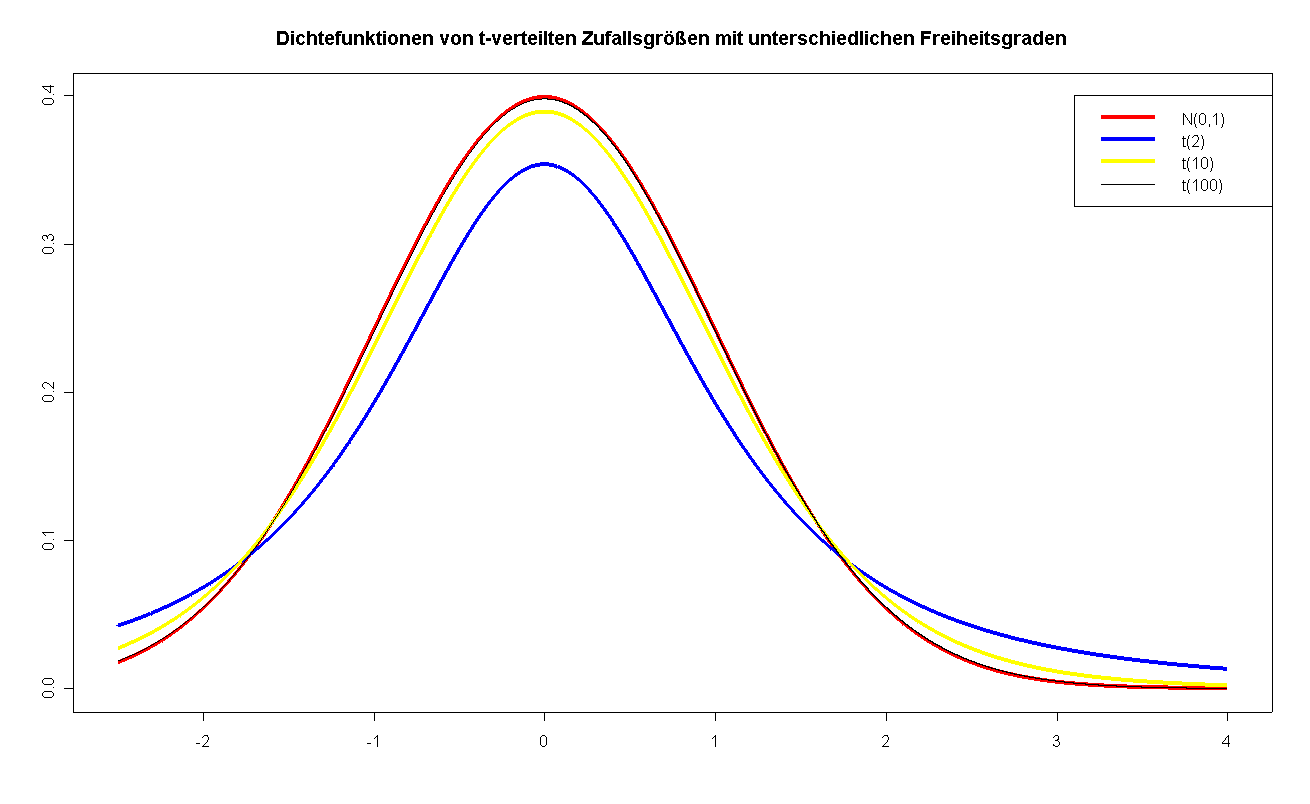
\includegraphics[width=8cm,height=4cm]{./bilder/T-Verteilung.png}\\
		$\lim\limits_{x\rightarrow \infty}$ = 0 aber langsamer wie bei
		Gaussverteilung 
    \end{minipage}

		\begin{tabular}{p{2cm}p{16cm}}
        Beispiel: & \textcolor{green}{10} Messungen ergeben Durchschnittswert
        \textcolor{red}{4{,}7} und eine Standardabweichung \textcolor{blue}{0{,}1}.
        Finde ein 99\%  Konfidenzintervall für $\mu$.\\
        
         Finde t: & \begin{tabular}{| c | c | c | c |}
                   \hline
                   $k=\textcolor{green}{n}-1$ & \ldots & 0{,}995\\
                   \hline
                   \vdots & \vdots & \vdots \\
                   \hline
                   9 & \ldots & 3{,}2498\\
                   \hline
                   \end{tabular}
        
       		 $\left[\textcolor{red}{\bar{X}}-3,2498\frac{\textcolor{blue}{S}}{\sqrt{\textcolor{green}{n}}},
		\textcolor{red}{\bar{X}}+3,2498\frac{\textcolor{blue}{S}}{\sqrt{\textcolor{green}{n}}}\right]
		\Rightarrow 
		\left[{\color{red}4{,}7}-3{,}2498\frac{\textcolor{blue}{0{,}1}}{\sqrt{\textcolor{green}{10}}},
		\textcolor{red}{4{,}7}+3{,}2498\frac{\textcolor{blue}{0{,}1}}{\sqrt{\textcolor{green}{10}}}\right]$\\ \\
		& $\mu\in \left[4{,}5072, 4{,}8028\right]$ mit Wahrscheinlichkeit 99\%
        \end{tabular}
\hrule

	\subsection{Konfidenzintervall \skript{139} \sachs{146}}
	\begin{tabular}{p{18cm}}
     Ein Intervall $[L(X_1,\ldots,X_n),R(X_1,\ldots,X_n)]$ heisst ein
     $1-\alpha$- Konfidenzintervall für den Parameter $\vartheta$, wenn der wahre
     Wert des Parameters $\vartheta$ höchstens mit Wahrscheinlichkeit $\alpha$
     ausserhalb des Intervalls liegt.
    \end{tabular}\\